\section{Results}
\label{sec:results}

The primary experiment is the Class~A search for a drifting, unresolved
carrier: \NWinA{} fine-channel windows toward \NSysClassA{} systems,
\EdrNWinA{} of them channelised finely enough to tell a drifting carrier from
a stationary one (\S\ref{sec:statistic}). The secondary Class~B search looks
for an unresolved spectral excess, with no discrimination by drift, in
\NWinB{} coarse windows. Together they make up the \NWindows{} windows of the
primary census.

\subsection{Sensitivity}
\label{sec:pninetysel}

Every Class~A limit in this paper has the same meaning. It is the
equivalent isotropic radiated power at which a carrier at the star, drifting
at a constant rate, makes a threshold crossing in nine trials in ten
($\mathrm{EIRP}_{90}$, Table~\ref{tab:quantities}), before the spatial rank
against the control positions is applied. A carrier whose drift rate
changes during the integration is not covered by that figure
(\S\ref{sec:excludes}). The Class~B limits are built in the same way, but
they are limits on an unresolved spectral excess, with no test of drift and
with an injection factor of their own (below).

For the median system, on its best window, a carrier of
$\EirpNinetySysMedA$\,W would make such a crossing nine times in ten. Of the \NSysClassA{} systems,
\NSysALostName{} has no limit at all, because every one of its windows lies
inside the line mask, and \OmNFlagWord{} more have limits that hold only if
their adopted positions are right. The median, and the counts that follow,
are therefore taken over the remaining \NSysALimSum, and the
\OmNFlagWord{} are described at the end of this section. Over these systems
the limits run from $\EirpNinetySysLoA$ to $\EirpNinetySysHiA$\,W
(Fig.~\ref{fig:classasens}), and \NSysEfifteen{} of them reach
$10^{15}$\,W. A single Class~A window is, of course, less deep than the best
window of a system, and the median window reaches
$\EirpNinetyWinMedA$\,W.

Each limit is taken over the channels that the line mask leaves free in the
star's own rest frame (\S\ref{sec:summary}), and this matters most for the
finest windows. The observers tuned these to CO, and a
\UmFineChanKHz\,kHz window spans only \UmFineBwMHz\,MHz, which is less than
the \UmFineMaskMHz\,MHz the mask removes about the line. Hence
\UmNWinAFull{} of the Class~A windows lie wholly inside the mask and
constrain nothing, which is why \NSysALostName{} has no limit. Using only the
\EdrNWinA{} windows fine enough to resolve a drift leaves a system's limit
\ScEdrMedClause.

The limits come from injection. Carriers were injected at a random
sub-channel phase, with a constant drift drawn from each window's own grid, and
recovered through the unchanged pipeline as far as the localisation at the
star. In a Class~A window without online spectral averaging, nine in ten
come back at $\IjFacNOne\,P_{\rm trig}$, where $P_{\rm trig}$ is the bare
$\LtCommonSnr\sigma$ of the window itself. With two-channel averaging the
figure is $\IjFacNTwo\,P_{\rm trig}$, and with averaging over four channels
it is $\IjFacNFour\,P_{\rm trig}$. That power is $\mathrm{EIRP}_{90}$.

The class-average factor of $\times\EirpNinetyMultA$ in
Table~\ref{tab:p90budget} is related to these, but it is never used on
its own. It was measured with the channel profile the injections deposited,
and each window's own response, measured on identical carriers, changes it
by $\times\IjRatioNOne$ without averaging and by $\times\IjRatioNTwo$ with
two-channel averaging. The limits use the window's own factor, so
$\times\EirpNinetyMultA$ is never applied to a window as it stands. The
factor shows no trend with the brightness of the control ring, so one value
can serve the whole class, while each window's own channel response is
carried by injections into the extraction that the search used
(Appendix~\ref{app:conventions}). Class~B has its own factor,
$\IjFacBNOne\,P_{\rm trig}$ ($\IjFacBNTwo$ with two-channel averaging),
measured with \SensNToneCoarse{} carriers injected into \SensNInjCoarse{}
coarse windows.

The calibration of the class factor is uncertain by
$\times\SensFacLo$--$\times\SensFacHi$ (Table~\ref{tab:p90budget}). This
interval applies to the median and to the counts, which are taken over
many windows. It places the median system between $\TfMedCalLo$ and
$\TfMedCalHi$\,W, so the second figure of the median is set by the
calibration.

Some windows already hold something above the trigger at the star, and
their limits are treated differently. This moves the best-window limit of
\XwNSysWord{} systems, \XwSysNames{} (marked \XwMark{} in
Table~\ref{tab:persys}), and \XwHeadlineClause. There are \XwNWin{} such Class~A windows, the \CeObs{}
that hold an unattributed crossing and \XwNWinSecWord{} more where only a
weaker cell, behind an attributed crossing, is unattributed. In them a
carrier that only just reached the trigger would not have stood out from
what is already present, so we quote instead the power at which nine
injected carriers in ten reach the window's own statistic, which lies
between $T_\star=\XwTobsLo$ and \XwTobsHi. None of these windows was itself
injected, so the figure is read from the pooled injections at that level,
and it raises their limits by at most \XwFacMaxPct{} per cent. Quoted in
this way, these limits err on the conservative side.

These limits describe the trigger completeness of the search, that is, the
chance that a carrier at the star makes a threshold crossing. The spatial
rank against the \NCtrl{} control positions is not charged against them,
because it decides only which crossings are examined first. A crossing that
fails the rank stays in the census, counts against the chance expectation
and goes on to the recurrence tests like any other (\S\ref{sec:summary}).
Charging the rank would raise the limits, by a factor that grows with the
brightness of the control ring. Appendix~\ref{app:persys} gives that cost
and its effect on the median and on the count at $10^{15}$\,W.

The largest caveat on these limits is that most of them are transferred
rather than measured. Carriers were injected directly into \SensNInj{} of
the \NWinA{} Class~A windows, \SensNInjPct{} per cent, and the result was
carried across to the other \SensNTransfer. The injected windows were whole
execution blocks, drawn at random and balanced by band and array, and they
resemble the population well. Their medians match to within
\RpCovOtherPct{} per cent on \RpCovOtherOf{} properties compared, and
differ by $\times\RpCovWorstRatio$ on the \RpCovWorstOrd, \RpCovWorstAxis.
Only the ninety per cent point, in units of each
window's own trigger power, is carried across. Among the injected windows
that point ranges from $\times\SensIndivFacLo$ to $\times\SensIndivFacHi$ of
the adopted factor, with \NmDispNTenth{} of the \SensNInj{} within a tenth of
it. This dispersion, and not the calibration interval, measures how
uncertain the limit of one uninjected window is.

Just \SmcNMeasSys{} systems had their best window injected directly, and
these are marked with a dagger in Table~\ref{tab:persys}. Most of the transferred windows,
\NgNInterpWin{} of the \SensNTransfer, lie inside the injected range on all
five of the properties that set the reading, and for a system whose best
window is one of these the headline limit is an estimate carrying that
dispersion. How much the dispersion matters for the sample as a whole is
shown in Appendix~\ref{app:persys} by redrawing the transferred factors at
random, and the median moves by only \SvRsMedShiftPct{} per cent.

The other \NgNExtrapWin{} transferred windows lie outside the injected range
on at least one property, where that range is not an empirical bound. In
all, \NgExtrapTakeClause, namely \NgExtrapSys, and these are marked with a
pilcrow in Table~\ref{tab:persys}. Their limits are extrapolations of the
injection calibration through a model, and not ninety per cent completeness
measurements bounded by injections, so the values quoted for them are best
read as approximate estimates of sensitivity. No measured dispersion is
attached to them. Since none of them is among the \NSysEfifteen{} reaching
$10^{15}$\,W, leaving them out does not change that count, and the median
over the other \NgNSysInterpSum{} systems is $\NgSysMedInterp$\,W.

A related caution applies to a star that lies far from the phase centre.
The injections were made at offsets of up to \OffInjMaxArcsec$''$ from the
phase centre, and the best window of \OffNames{} puts the star well beyond
that, where the primary-beam response is below \OffAcut. Its limit rests on
the model of the beam alone, with no injected configuration behind it, and
it carries the mark \OffMark{} in Table~\ref{tab:persys}. Pointing errors
also matter most there, because the response falls most steeply far from
the centre: the pointing term of Table~\ref{tab:p90budget} is
\PtUncDeepPct{} per cent for that window, against \PtUncMedPct{} per cent
for the median window. The deepest limit that does rest on injected
configurations is $\PtDeepInjEirp$\,W, toward \PtDeepInjStar.

Two further effects lie outside the injections. The first is atmospheric
decorrelation, which a real carrier suffers and an injected one does not.
It is estimated from each block's phase-calibrator phase rms
\citep[\S\S10.4.11, 11.3.1]{ALMAHandbook} with the phase-scatter relation of
\citet[Eq.~3]{Richards2022}, and the adopted limits have it divided out. The
phase rms is recorded for \SensDecorNBlk{} of the \SensDecorNBlkTot{}
blocks, and there the correction is measured. For the others it is
imputed, as \DcImputedRule, and applied in the same way, and these are
marked in Table~\ref{tab:persys}. Only the one system with neither keeps
its uncorrected value. For most systems the
correction is small, \NmDecSysMedPct{} per cent for the median system's
best window, but it exceeds a tenth for \NmDecNBigSys{} of the \NSysALimSum{} systems and reaches
\NmDecSysWorstPct{} per cent for \NmDecSysWorstName. Without it the median
limit would be $\DcSysMedNom$\,W and \DcNomNEfifteen{} systems
would reach $10^{15}$\,W.

The correction is itself a floor. The phase rms is measured on the
calibrator, which lies some way from the star and is observed only between
target scans, so it misses whatever phase noise is particular to the
star's own line of sight. The adopted limits are therefore still optimistic
by any decorrelation that the calibrator does not see. The channel response,
online spectral averaging included, is by contrast measured and applied.

The second effect is the position of the star itself. For \OmFlagStars{} the
astrometric solutions are disturbed, and there is neither a companion nor a
Hipparcos epoch with which to correct them
(Appendix~\ref{app:conventions}), so the amplitude lost at the adopted
position has no bound. Their limits in Table~\ref{tab:persys} hold only if
that position is right, and these \OmNFlagWord{} systems are left out of the
median, the count at $10^{15}$\,W and Fig.~\ref{fig:classasens}.

A carrier that is not always radiating is penalised in proportion. In
\DutyNTrial{} undrifted trials down to a \DutyCycleMinPct{} per cent duty
cycle the recovered amplitude followed the duty cycle to within
\DutyAttenDevPct{} per cent, so a transmitter that is on for a tenth of the
time would need $\DutyPowFac\times$ the power quoted. The drifting,
intermittent case has not been measured.

Two of the nearest stars appear only in the secondary search. Barnard's
Star and Wolf~359, the second- and third-nearest stellar systems once brown
dwarfs are set aside, were not targets of the \SbPriorFreqGHz\,GHz searches
of \citet{Steffes1994} and \citet{Mauersberger1996}, and have otherwise been
searched at centimetre wavelengths \citep{Enriquez2017,Price2020,Margot2023}.
The archive holds only coarse Band~6 windows toward them, so their values,
$\EirpNinetyBarnLo$--$\EirpNinetyBarnHi$\,W over \NWinBarn{} windows and
$\EirpNinetyWolfLo$--$\EirpNinetyWolfHi$\,W over \NWinWolf, are limits on an
unresolved narrowband spectral excess, and to our knowledge the first at
millimetre or submillimetre wavelengths for either star.

No Class~B window that passes the quality criterion holds a crossing, which
is what chance predicts. Computed exactly as for Class~A, the
\CeNWinBClean{} windows expect \CeExpB{} crossings from their own control
positions ($P(0)=\CeProbZeroB$). The expectation is small because a coarse
window holds a median of only \CeIndCellsMedB{} independent cells, against
\CeIndCellsMedA{} in Class~A.

\begin{table*}
\centering
\scriptsize
\caption{What sets $\mathrm{EIRP}_{90}$, and in which direction. The
calibration interval applies to the class-average factor and so to many
windows, the spread between windows to one window. Pointing is a per-window
uncertainty; the decorrelation left after correction is one-sided.
Retentions are listed below the table (\S\ref{sec:pninetysel}).}
\label{tab:p90budget}
\setlength{\tabcolsep}{2pt}
% GENERATED by sens_r11.py -- do not hand-edit.
\begin{tabular}{@{}l@{~~}r@{~~}>{\raggedright\arraybackslash}p{0.61\linewidth}@{}}
\hline
 & value & what it does to the limit \\
\hline
Class-average completeness & $\times2.99$ & nine carriers in ten recovered at this multiple of a window's own trigger power, with the deposited channel profile. \emph{Measured} in the 49 Class~A windows injected directly and \emph{estimated}, at this factor, in the other 356 \\
Own channel response & $\times\IjRatioNOne$, $\times\IjRatioNTwo$ & the ninety per cent point with the window's own response, online spectral averaging included, over that with the deposited profile, without and with two-channel averaging ($N=1$, $N=2$; $\times\IjRatioNFour$ at $N=4$). \emph{Measured} on identical carriers in \IjNWinA{} Class~A windows and \emph{applied}: a window's factor is $\times\IjFacNOne$ or $\times\IjFacNTwo$, and $\times\IjFacNFour$ in the one window averaged over four channels \\
Calibration interval & $-11/+11$\,\% & $\times0.89$--$\times1.11$ on the factor, and so on the median limit and the system counts. Combined in quadrature from the factor's sampling error over the 49 injected windows ($\pm2$ per cent), the observatory's band-dependent flux-scale specification (\BudFluxSource; \BudFluxSpec, $\pm\BudFlux$ per cent weighted over this sample's bands) and the distance and visibility scale ($\pm\BudDistVis$ per cent); $\pm\BudCombWorst$ per cent for the \BudNHiWin{} Class~A windows in \BudHiBandWord~\BudHiBands, at \BudHiGHzList\,GHz \\
Window to window & $\times0.81$--$\times1.12$ & an observed dispersion, not an error bar: the 49 injected windows resolve 2.41--3.36\,$P_{\rm trig}$ individually, \NmDispNTenth{} of them within a tenth of the pooled value. This, and not the interval above, is what an estimated limit is uncertain by; it is wider. It applies to the \NgNInterpEstSysBnd{} transferred limits inside the injected configurations, not to the \NgNExtrapSysBnd{} outside them \\
Pointing & $\pm0$--$\PtUncMaxPct$\,\% & an uncertainty, not applied: the slope $|{\rm d}\ln A/{\rm d}\theta|=8\ln2\,\theta/\theta_{\rm PB}^{2}$ of the primary beam at the star's offset $\theta$ times ALMA's offset-pointing accuracy, \PtSigmaOff$''$ rms in every band \citep[\S10.3.3, App.~A.1]{ALMAHandbook}. Zero at the pointing centre; $\pm\PtUncMedPct$ per cent in the median Class~A window and $\pm\PtUncSysMedPct$ on the systems' best windows; $\pm\PtUncDeepPct$ per cent on $\epsilon$~Eridani's, $\pm\PtUncDeepAbsPct$ at the \PtSigmaAbs$''$ all-sky accuracy \\
Decorrelation & $+0/+\NmDecSysWorstPct$\,\% & \emph{applied}, window by window: estimated from the phase rms the observatory records on each block's phase calibrator, which an injected carrier does not suffer and a real one does. \emph{Measured} where the delivery records it (\SensDecorNBlk{} of the \SensDecorNBlkTot{} blocks) and \emph{imputed} from blocks matched in baseline length where it does not. A median $+\NmDecSysMedPct$ on the systems' best windows, $+\SensDecorHiPct$ above \SensDecorHiGHz\,GHz, and more than $+\SensDecorTailLevelPct$ in \SensDecorTailPct{} per cent of windows. The correction is itself a floor, so the limits stay optimistic, one-sidedly, by any decorrelation the calibrator does not see \\
\hline
\end{tabular}
\par\smallskip\raggedright\emph{Applied window by window, and so not part of the budget} (Appendix~\ref{app:conventions}): the intra-integration smearing, $\times1.00$--$\times\SmcFacWorst$, from each window's own integration length where it is recorded (\SmcNMeas{} windows) and bounded where it is not (\SmcNBound); the primary-beam response at the star's offset, $\times1.00$--$\times\NmBeamFacWorst$, with a one-sided model departure of up to \BmModelMaxPct{} per cent in the \BmNAboveTenPct{} windows furthest off-axis; and the annual parallax, $\times1.00$--$\times2.06$, only where a product predates the extractor that centres it on the star's apparent position (\PxaNWinARet{} Class~A windows; bounded on the \PxaNMissing{} with no parallax record).

\end{table*}

\begin{figure}
\centering
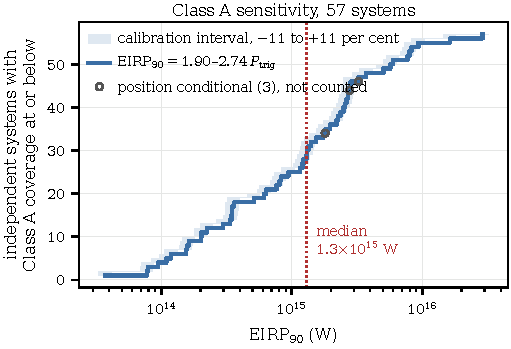
\includegraphics[width=\columnwidth]{figures/classa_sensitivity.pdf}
%% ★ r27 (R2-D10): panel (b), the Class A systems with a separated repeat
%% counted by system, duplicated Fig.~\ref{fig:confcov}b and LEAVES; Fig. 5
%% itself is protected and stays, one panel, one column.  Its four assertions
%% (\ZcConfSysDay, \ZcConfSysYr, \ZcNoRepSys, NSysClassA) still run in
%% make_fig_classa_sens.py.
\caption{\textbf{Single-epoch trigger completeness of the carrier search}:
the cumulative number of systems whose best window reaches a given
$\mathrm{EIRP}_{90}$, decorrelation divided out, over the \NSysALimSum{} of
the \NSysClassA{} systems with a limit and a bounded position
(\S\ref{sec:pninetysel}), the calibration interval of
Table~\ref{tab:p90budget} shaded. No power buys a separated repeat at the
same frequency, which \ZcNoRepSys{} systems lack
(Fig.~\ref{fig:waterfall}b; \S\ref{sec:mmdifferent}).}
\label{fig:classasens}
\end{figure}

\subsection{Threshold crossings}
\label{sec:technosearch}

Of the \NWindows{} windows of the primary census, \CsNCross{} hold a cell
reaching $T\geq\StageNullTrig$ at the stellar position, all in data that pass
the quality criterion of Appendix~\ref{sec:blockquality}. The window flag of
that appendix reaches \DqNWin{} windows in \BkFlagNBlock{} blocks, and the
\BkFlagNCrossOtherWord{} crossing it reaches, toward \BkFlagOtherStar, is
withheld from the tests that depend on amplitude. The
$\pm\MaskHalfKms$\,km\,s$^{-1}$ line mask places \MkNCoinc{} of the
\CsNCrossQp{} within that velocity of a catalogued transition in the star's
own rest frame (Appendix~\ref{app:linemask}). Those \CsNAttrQp{} are
attributed, \LnAttrSupp{} with corroborating evidence of line emission and
\LnAttrCoinc{} on the coincidence alone, and \CsNUnattrQp{} are
unattributed. None was identified as interference by the available
diagnostics (Appendix~\ref{app:rfi}). The archival tail adds
\CeNTailCrossWord{} more, both unattributed and both toward \CeTailStar, in
windows that no expectation covers (Table~\ref{tab:blockledger}). They are in
the ledger, but in none of the counts above. The correlator's frame
suggests that the attributions reflect line emission, and not merely the
width of the mask, since in that frame the crossings crowd onto the
transitions these setups were tuned to (Appendix~\ref{app:rfi}).

Of the \CsNCrossQp, \LrStageN{} outrank all \NCtrl{} control positions of
their own window, and \LrStageNCo{} of these are carbon monoxide,
\JqNBpCoWord{} toward $\beta$~Pic and \JqNHdCoWord{} toward HD~48370.
$\beta$~Pic has \BpicPanelNCo{} CO crossings in the census in all, so
\JqNBpCoWord{} of them outrank every control position and the remaining
\JqNBpCoOutWord{} is outranked by its own bright control ring. The
other crossing to lead its field, toward \EvAStar, is the only unattributed
crossing to do so. It is not present again at its own frequency in the
star's frame (\S\ref{sec:vistest}). Behind the
windows' largest cells, \CkNSecondaryWord{} weaker cells in all also reach the
trigger. Of these, \CkNSecUnattrWord{} are unattributed, against \AcSecExp{}
expected from the control positions (\S\ref{sec:trigunif}), and \CkNRecurWord{} reaches the
trigger in any covering block the recurrence test reads. None of the unattributed
crossings is found again as a recurrent feature (\S\ref{sec:etacrv}), and
this survey reports no detection; the deposited crossing ledger lists every
one.

\subsubsection{How many crossings chance predicts}
\label{sec:trigunif}

We first ask whether the unattributed crossings are more numerous than
noise alone would give. The number of searched channel\,$\times$\,drift
cells in a window spans \TuCellsDecades{} decades, so the expectation is
built window by window over the \CeNWin{} Class~A windows of the census,
from each field's own control positions. The same condition is applied on
both sides. A window counts once, by \AcRulePrimary, when that cell
reaches the trigger and the line mask does not attribute it, and a control
position counts by its own largest cell in the same way
(Appendix~\ref{app:falsealarm}). The control positions predict \CeExp{}
unattributed Class~A crossings, and \CeObs{} are found. A count that large
or larger arises by chance with probability \CeProbNull.

The rule matters. If a window counts instead whenever any of its cells above
the trigger is unattributed, \AcObsWin{} are found against \AcExpWin{}
expected ($P=\AcProbWin$). If every such cell counts, at the star and at
the control positions alike, \AcObsCell{} are found against \AcExpCell{}
($P=\AcProbCell$). Doubled for the choice between counting the largest cell
and counting every cell, this is \AcProbCellTwoPhrase; trebled for all three
rules compared, it is \AcProbCellThree. The difference lies in the weaker
cells. The
stars carry \AcStarSecNWord{} unattributed cells behind their largest, where
the control positions predict \AcSecExp{} ($P=\AcProbSec$). These lie in
fields with known line emission or already among the crossings, and none of
them is found again in another block (\S\ref{sec:etacrv}). The stellar
position also carries continuum and line emission that its controls lack,
and calibrated at the star's own excess over its controls just below the
trigger (below), the every-cell probability becomes \AcProbCellNear.

The part of the expectation that the mask removes is also taken window by
window, from the share of each window's own control maxima that land on
masked channels. Where a window has only a few such maxima, its share is
drawn toward the share pooled over all windows (Appendix~\ref{app:falsealarm}).
A single pooled share, applied to every window alike, serves as the check,
and gives \CeExpPool{} expected ($P=\CeProbNullPool$). The per-window figure
is \CeExpMovePool{} lower because the line-rich windows, where the controls
trigger most often, also put more of their maxima on lines.

That probability, and the others built from the control positions here and
in \S\ref{sec:etacrv}, rest on two conditions. The first is that the control
positions are a fair model of the background at the stellar position. The
searched data cannot test this. A residual of calibration or imaging that
raised the rate of crossings at the star without raising it at the controls
would change the probabilities, and a calibration error that varied with
frequency is one such residual, since it would raise the star and not its
continuum-free controls. To make a crossing on its own it would need
\CyEpsMinPct{} per cent of the star's continuum even in the least demanding
window, but a smaller residual adding to the noise could still change the
rate. As a sensitivity check, the stellar rate can instead be calibrated at
the ratio \CeNear{} that the star shows over its controls just below the
trigger, and the expectation is then \CeExpNear{}, at $P=\CeProbNear$.

The second condition is the mask itself. Its species list was completed
after the crossings had been examined, and SO was added after a crossing had
been found on one of its lines (Appendix~\ref{app:linemask}). The
probabilities, and the allowance given below, are therefore conditional on
the mask as adopted. Without SO the same comparison gives \MkNoSOObs{}
observed against \MkNoSOExp{} expected, at $P=\MkNoSOProb$.

The expectation is not carried by a few noisy fields. Without the
\BgTopNWord{} windows whose control positions trigger most often, the
remaining \BgDropTenNWin{} predict \BgDropTenExp{} against \BgDropTenObs{}
observed. In \BgConfInOf{} subsets by band, array, channel
width and field type, the observed count lies within the central
\CeCovPct{} per cent of its own predicted distribution.

Both sides of the comparison are read over the whole primary beam, the field
of \S\ref{sec:statistic}. The extraction's original rule was narrower,
keeping only the one field entry whose phase centre lies nearest the star,
which drops on-source time and real signal. Neither rule has an adjustable
radius. Read over that narrower field on both sides, the comparison gives
\FrNarrowObs{} against \FrNarrowExp{}, at $P=\FrNarrowProb$. Neither geometry
was nominated as the primary before the counts were seen.

Because the field and the mask were both chosen after the crossings were
seen, the comparison was repeated for all \CgNCellWord{} combinations of
field, mask and background rate (Table~\ref{tab:choicegrid},
Appendix~\ref{sec:choicegrid}). The smallest probability among them is
\CgMinProb, for \CgMinCell. Because it was picked as the smallest
of the \CgNTrialWord{} combinations of field and mask that were examined,
it is multiplied by \CgNTrialWord, which gives a value \CgBonfPhrase,
\CgVerdictClause. That factor allows for this one choice and for no other
taken after the crossings were seen, and the probability still rests on the
control positions being a fair model of the background.

The comparison can also be read the other way, as a measure of how much
larger the background could be before the observed count became improbable.
If \CeAddLim{} is added to the mean number of crossings expected from the
control positions, a count as low as \CeObs{} still has a probability of
\CeProbAtLim, above the one-sided \CeAlphaPct{} per cent level, while one
more brings it to \CeProbAboveLim, below that level. Read over the nearest field only, the
figure is \FrNarrowAddLim. This is a statement about the mean of
the background model, and it carries the same two conditions as the
probability. It is not a confidence bound on how many of the observed
crossings are real, and still less a count of transmitting systems or an
occurrence rate (Appendix~\ref{app:falsealarm}).

Broadband continuum flares from the stars can be excluded as an
explanation of the narrow-channel crossings. A millimetre flare raises every
channel of a window alike, so one able to make a single-channel crossing
would appear as a \FlPredLo--\FlPredHi$\sigma$ continuum event in the same
integrations. The observed continuum statistic of the crossings, by
contrast, has a median of \FlObsMed, and the \FlEgStar{} flare of
\citet{MacGregor2020}, in a block that also holds a crossing, adds only
\FlEgContrib$\sigma$ to the single-channel statistic. This test says nothing
about stellar emission confined to a narrow range of frequency, although
nothing found here points to such an origin for any of the unattributed
crossings.

\subsection{$\beta$~Pictoris: the positive control}
\label{sec:bpicval}

A search that finds nothing must show that it could have found something,
and $\beta$~Pictoris provides that test. Without being told the disc is
there, the pipeline recovers its circumstellar carbon monoxide
\citep{Dent2014,Matra2017} in two rotational transitions, in
\CsBpCoBlocks{} execution blocks drawn from \CsBpCoSess{} observing sessions
over \BpBaselineYr\,yr. In the star's rest frame, at each block's own epoch,
all \BpicPanelNCo{} of its CO crossings lie within \BpicDvCoHi\,km\,s$^{-1}$ of the
adopted systemic velocity. That velocity, however, was itself measured from
ALMA observations of the same CO \citep{Matra2017}, so the agreement checks
the registration from one epoch to the next, and it cannot check the
absolute frame.
The \LrBpNVel{} velocities have a standard deviation of
\LrBpDvSd\,km\,s$^{-1}$ and a full spread of \LrBpDvRange\,km\,s$^{-1}$. The same emission is the positive control of the
line-recurrence check of \S\ref{sec:etacrv}: every feature recurs in another
execution block, and each transition in another session. Emission of this
kind is what the line mask removes, including the CO(2--1) toward
HD~48370 that \citet{Cataldi2023} report and flag as possible cloud
contamination (Appendix~\ref{app:linemask}). The mask covers \FrNSpec{}
species and costs \MkMaskAPct{} per cent of the Class~A union bandwidth, and
it is the single most productive test in the chain
(\S\ref{sec:mmdifferent}).

\subsection{Candidates and recurrence}
\label{sec:etacrv}

\phantomsection\label{sec:vistest}%
\emph{The field leader.} One unattributed crossing has a stellar statistic
above every one of the \NCtrl{} control positions in its own window: the one toward
\EvAStar{} at \RqFreqSx\,GHz, in Band~\EvABand{} and in the star's own rest
frame (Table~\ref{tab:cand}; Fig.~\ref{fig:event}). The rank decides which
crossings are examined first, and on its own it disposes of nothing
(\S\ref{sec:summary}). If the stellar and control positions were
exchangeable, the control ensembles would predict \RkCondExp{} unattributed
census crossings leading their field by chance, and \RkCondNObsWord{} or more
with probability \RkCondProb. In the reserved blocks \RkHoLeadWord{} of the \RkHoNWord{}
crossings leads its field, and beyond 40\,pc \RkOosLeadWord{} of the \RkOosNWord{} does. A
visibility-domain fit was made for \CsNVisFit{} of the \CsNCross{} census
crossings, and for \CsNVisLocal{} of them it is consistent with a point source
at the star. Of the other \JqNNotLoc, \JqNNotLocUnWord{} is unattributed and
\JqNNotLocCoWord{} are $\beta$~Pic's CO(1--0), which the array resolves.
Of the \JqNUnfit{} never fitted, \JqNUnfitLateWord{} lie in blocks that the
fitting campaign did not include, \JqNUnfitNocalWord{} in blocks it could not
calibrate and \JqNUnfitOtherWord{} in blocks fitted at another cell, and
\JqNUnfitUn{} of them are unattributed. The unattributed crossings among
these stay in the comparison with chance, because the control positions
they are compared with are not localised either. The fit
does not reject the field leader, and injected point sources in
the same bin return ${\rm Re}/\sigma=\RsevReAtFiveMeanA\pm\RsevReAtFiveSdA$.

The star has been observed again at the same stellar-frame frequency in a
separated session, and \RcSxSepClause. The carrier's own fitted drift would
take it out of that half-channel cell ($\pm\RqDispSx$\,km\,s$^{-1}$) in
\ZtSxLeaveSec\,s, so the repeat reading is the line-recurrence check of
Table~\ref{tab:quantities}. At the nominal threshold-equivalent amplitude
$5S/T_\star$ the separated blocks would recover such an emitter with
calculated probability \RcSxPowerTrig, conditional on that amplitude, and
injected carriers measure \HjMeasSx. In Table~\ref{tab:cand}, $T_{\rm rep}$ is one cell
at one trial and may be negative, and the recovery chance in brackets, at the
discovery amplitude, is biased high. The readings behind each bound are in
\texttt{candidates/repeat\_epoch\_readings.csv} of the data archive
\citep{SIdeposit}. Of these blocks, \RcSxNDeepWord{} were taken in
\RcSxDeepYears, \RcSxDeepSepD{} days before the discovery, and they reach
\RcSxDeepSigLo--\RcSxDeepSigHi\,mJy per channel at the predicted cell,
against an amplitude uncertainty of \RcSxFluxErr\,mJy in the discovery
block\RcSxLimClause.
%% r36 R2-1 (N1 hook 1): the deep 12-m blocks are recurrence readings; Table F1 note says why 61 Vir's limit is deep.

\emph{The predicted cell.} The same check, applied to every crossing, reads
the one cell each discovery predicts at its nearest separated repeat. It
works on lines, since \MkAttrRecur{} of the \MkAttrTested{} attributed
crossings tested recur in another session, \QcSepMinD--\QcSepMaxD\,d away, and the
\MkAttrExcl{} that do not are the faintest of them. Of the
\MkUnattr{} unattributed crossings of the \NtSetUnName, \RcNExclPoss{} could
be read at their predicted cell, and on these it
returns nothing. The
largest readings are \RcTMatched{} at the carried drift and \RcTMax{} at any
drift, against a trigger of \StageNullTrig. For \RcNFracBelow{} of the
\RcNExcl{} the repeat bounds a line-like emitter returning to its cell
below the discovery amplitude, at a median \RcFracMed{} of it. At the
weaker nominal threshold-equivalent amplitude, \HjNPowerLo{} of the
\RcNExcl{} are too shallow to test. A drifting
carrier, on the other hand, would not stay in that cell, so this null speaks
only to an emitter that holds a stationary frequency in the star's frame. The
bounded crossings accelerate at \ZtALosLo{} to \ZtALosHi\,m\,s$^{-2}$
(\EgExStarALosLo{} to \EgStarALosHi\,m\,s$^{-2}$ in the star's frame), so a
carrier leaves its half-channel cell within \ZtLeaveSecLo--\ZtLeaveSecHi\,s,
far sooner than the nearest covering block comes round. Nor can the check be turned into a test of a
drifting carrier by carrying the fitted drift forward, since the drift's own
resolution moves the predicted cell by a median \ZtRegChanMed{} channels by
the nearest repeat. A drifting carrier is tested instead by the widened
window and the pair test below. No bound depends on the
cell's registration, the anchor or the threshold
(Appendices~\ref{sec:nullscatter} and~\ref{sec:regbudget}).\RcNoRepeatSentence{} None of the unattributed crossings is therefore a recurrent
feature in the sense of Table~\ref{tab:quantities}, which is only the first
of the requirements that table sets for an artificial origin.

\emph{The widened window.} A transmitter in orbit changes its line-of-sight
velocity between epochs, so the broadest reading asks whether anything
reaches the trigger, at any drift, anywhere in a covering window of a
separated session. In the median case that window is
$\pm\WdHalfKms$\,km\,s$^{-1}$ wide. Of the \WuNWin{} distinct covering
windows, \WuNWinExc{} hold a statistic above the trigger, against the
\WuExpWinCtrl{} that each window's own control positions predict
($P=\WuProbWinCtrl$; Appendix~\ref{app:falsealarm}). Every one of those
windows holds a crossing the ledger already lists, so the comparison
re-reads the trigger-level count of \S\ref{sec:trigunif} rather than adding
a recurrence to it. Of the \WuNWinExc, \WuNWinExcTwo{} are toward
\WuTwoStars, which are also the two most heavily observed objects in the
survey: they hold \TwWinASharePct{} per cent of the Class~A census and
\TwNWinTwo{} of the \WuNWin{} covering windows, so \TwExpTwoCtrl{} of the
\WuExpWinCtrl{} expected exceedances are theirs before anything is looked
at. Over the remaining \WuNWinRest{} windows the reading is
\WuNWinRestExc{} against \WuExpRestCtrl, at $P=\WuProbRestCtrl$.

\emph{The pair test.} A carrier that moves might also be caught as two
crossings toward one star, and Table~\ref{tab:pairs} asks of the \TjNPair{}
pairs inside the widened window, across \TjNStarPair{} stars, whether one
transmitter could have produced both. Constant line-of-sight acceleration
would require equal drift rates, and the fitted rates differ by more than the
grid's resolution in \TjUneqDriftOf{} pairs, so the question
becomes a weaker one: whether any trajectory inside the searched grid joins
the two. It rejects \TjNExcl{} of the \TjNPair. Of the \TjNOpen{} it
cannot reject, \TjOpenEdgeClause. An open pair is not a confirmation, since the
comparison can reject an association but cannot accept one
(\S\ref{sec:summary}). Chance alone, at each census window's own control
rate, would put \OpExpSepRange{} open pairs in separated sessions against the
\OpObsSep{} observed, with the pairs that have an archival-tail member set
aside. Of random pairs, \OpJoinPctLo--\OpJoinPctHi{} per cent are
joinable. As a test of a drifting carrier it is therefore incomplete.
Counting archival-tail blocks, \OpNTriAllWord{} star, \OpTriStars, has three
separated crossings that one trajectory joins pairwise, and in the census
alone \OpNTriCenWord{} does. However, no constant acceleration or circular
orbit inside the grid joins all three. Predicted from the first two, the
third misses a constant acceleration by at least
\TrAMissMin{} resolutions, and the best circular orbit through all three
misses by \TrJointMissMin. A line that does not drift behaves as it should
under the same test: the \TjCtlLine{} line of \TjCtlStar{} is joined across
\TjCtlDtD\,d to within \TjCtlNSig{} of the resolution. The accounting for
each pair is
\texttt{candidates/\allowbreak drift\_pair\_accounting.csv} of the data
archive.

\phantomsection\label{sec:twostars}%
\emph{HD~14055 and \BkAlmaName.} HD~14055 holds \TwNExcHD{} of the
exceedances against \TwExpCtrlHD{} expected ($P=\TwProbCtrlHD$), so its
concentration is its exposure. Its fields are ordinary, with control rings
\TwRingQHD{} times their class median against \TwRingQSurv{} for the survey.
Each of its \LrHdNBlk{} census blocks pairs \LrHdNCoarse{}
\LrHdCoarseChanMHz\,MHz continuum windows with \LrHdNFine{}
\LrHdFineChanKHz\,kHz windows, and all \LrHdNCross{} of its crossings lie in
fine windows that hold the \LrHdFineLines{} lines, \TwHDMaskLo--\TwHDMaskHi\,km\,s$^{-1}$ from the nearest masked
transition in its own frame. Two of its crossings were followed up in depth, by blocks outside the
census. For the first, the \TwHDNDeepSepFirst{} follow-up blocks in separated
sessions read \TwHDRepFirst\,mJy for a line-like emitter at the predicted
cell, against a discovery amplitude of \TwHDDiscFirst\,mJy, which bounds it
at \TwHDFracFirst{} of the discovery. For the second, \TwHDNDeepSepSecond{}
such blocks read \TwHDRepSecond\,mJy against \TwHDDiscSecond\,mJy, a bound
of \TwHDFracSecond.

\BkAlmaName{} is a serendipitous dwarf \TwPbJx{} arcsec from the phase
centre of fields pointed at the Lupus clouds, observed in \TwOnSrcJx\,s
snapshots. It holds \TwNExcJx{} exceedances where \TwExpCtrlJx{} were
expected, with $P=\TwProbCtrlJxRaw$ for this object alone. That probability,
however, belongs to an object picked out because it is the most discrepant of
the \TwLookNStarCtrl{} objects compared, and in Poisson-binomial counts
simulated at each object's own per-window control rates some object is that
far out in \TwLookPctCtrl{} per cent of realisations. Its
\TwNExcJxWord{} exceedances lie on \TwJxNCrossExcWord{} crossings between
\TwJxExcBandLo{} and \TwJxExcBandHi\,GHz, in \TwJxNBlockExcWord{} of this
object's \TwJxNBlockWord{} blocks, and their control rings are ordinary.
Their fitted drifts lie \TwJxStepLo--\TwJxStepHi{} grid steps from zero,
against an uncertainty measured by injection of at most \TwJxStepErr{} step.
Because the snapshots are spread over a \TwJxSpanS\,s track,
$\eta_{\rm drift}$ is \TwJxEtaSpanRange{} over the track and \TwJxEtaOnRange{}
over the time on source.

The star's offset from the phase centre is comparable to the synthesised
beam, so emission there could in principle reach the star's position. To test this, the
\TwJxNBlockExcWord{} blocks that hold the exceedances were re-calibrated,
which reproduces their \TwJxNCrossExcWord{} crossings exactly. The field at
the phase centre shows no line in the crossing channels, and the snapshot beam
is at most \JrBeamAbsMax{} at the star's offset. Whatever lies at the phase
centre, weighted by that beam, would add at most \JrLeakTMax{} to the
statistic of any crossing, against a trigger of \StageNullTrig. Leakage from the phase
centre is therefore excluded. A visibility fit along each crossing's own drift places
all \TwJxNCrossExcWord{} at the star (${\rm Re}/\sigma=\JrVfReLo$--$\JrVfReHi$,
Table~\ref{tab:jxfit}). The archived fits that placed
\JrVfNWrongDriftWord{} of them away from the star had followed the drift of
the other crossing in the same block.

Nor is a molecular line an obvious explanation. Only the attributed CO
crossing lies at the velocity of the Lupus molecular gas in the local
standard of rest (Appendix~\ref{app:linemask}), and in that frame none of
the \TwJxNCrossExcWord{} lies within \JqLineMinDv\,km\,s$^{-1}$ of the cloud velocity for
any of the \JqLineNList{} dense-gas transitions of DCO$^+$, DCN,
c-C$_3$H$_2$, CH$_3$OH and HC$_3$N in these windows. A wider list of
\TwWideNSpecies{} species places a transition within
\TwWideDvMax\,km\,s$^{-1}$ of every crossing toward either object, as its
\TwWideNTrans{} transitions guarantee, and so identifies nothing. We have no
explanation for these crossings, which lie at the star, are not leaked from
the field and do not fall at the velocity of any listed line of the cloud.
\BkAlmaName{} is a target for follow-up, not evidence of a
non-astrophysical source, and a repeat observation should point at the
star, with a radial velocity and one deeper epoch at
\TwJxExcBandLo--\TwJxExcBandHi\,GHz.

\begin{table}
\centering
\scriptsize
\caption{\textbf{The crossings toward \BkAlmaName.} Visibility fit at
the star and offset of the statistic's peak (\S\ref{sec:twostars}).}
\label{tab:jxfit}
% GENERATED by jx_r35.py (round 3520) -- do not hand-edit.
\setlength{\tabcolsep}{3pt}
\begin{tabular}{@{}rrrrrcr@{}}
\hline
$\nu$ & $T_\star$ & Re/$\sigma$ & Im/$\sigma$ & ctrl & at star$^{a}$ & peak$^{b}$ \\
GHz & & & & & & arcsec \\
\hline
216.184 & 5.25 & 4.1$^{c}$ & $-$0.9 & 1.8 & yes & 0.4 \\
217.729 & 5.09 & 4.3$^{c}$ & 0.4 & 0.8 & yes & 0.9 \\
218.671 & 5.05 & 4.5 & 0.5 & 1.5 & yes & 0.8 \\
218.873 & 5.11 & 4.7 & 0.1 & 1.1 & yes & 0.8 \\
230.522$^{d}$ & 5.39 & 4.4 & 1.0 & 3.3 & yes & 2.4 \\
\hline
\end{tabular}
\par\smallskip{\footnotesize\raggedright Re/$\sigma$, Im/$\sigma$: the mean real and imaginary parts of the visibilities phased to the star; ctrl: the largest Re/$\sigma$ at the fit\textquoteright s control positions and frequencies. $^{a}$Re/$\sigma\ge4$, $|$Im/$\sigma|<3$ and above every control. $^{b}$Distance from the star of the largest statistic on the search\textquoteright s source grid, which extends 3.0\,arcsec from it. $^{c}$Fitted along the window\textquoteright s own drift on the re-calibrated block; the archived fit had used the other window\textquoteright s. $^{d}$The CO($2{\to}1$) crossing, attributed.\par}

\end{table}

\phantomsection\label{sec:holdoutsearch}%
\emph{Blocks outside the census.} Three sets of execution blocks enter no
census statistic (Table~\ref{tab:blockledger}), and each was searched with
the same pipeline. The reserved hold-out, set aside by the identifier rule
of Appendix~\ref{sec:heldout}, has \HoNWin{} windows toward \HoNStar{} stars
and holds \HoNCross{} crossings, the strongest at $T_\star=\HoTMax$. Of the \HoNTested{} read at their predicted
cells, only a molecular line is present again ($T_{\rm rep}=\HoRecTRep$).
Compared with chance in the same way, its
\CgHoNWin{} fine-channel windows expect \CgHoExp{} unattributed crossings and
hold \CgHoObs{} ($P=\CgHoProb$). Its crossings were listed in the same session as the species-list query of
\MkListDate, so the record cannot tell whether they were seen before the
mask was completed, but no unattributed one lies within
\CgHoMinDv\,km\,s$^{-1}$ of a listed transition, and the later decision on
SO changes none of them (Appendix~\ref{app:radius}). The
archival extension's \LdgExtWin{} windows in \LdgExtEB{} blocks hold
\QxObsCross{} crossings, \QxObsUnattr{} of them unattributed against
\QxLam{} predicted by chance ($P=\QxPGe$). The control sample beyond
40\,pc holds \OosNCross{} crossings. Read in the sky frame it supports no
limit, and shows only that the pipeline behaves in the same way beyond the
sample.

\begin{figure*}
\centering
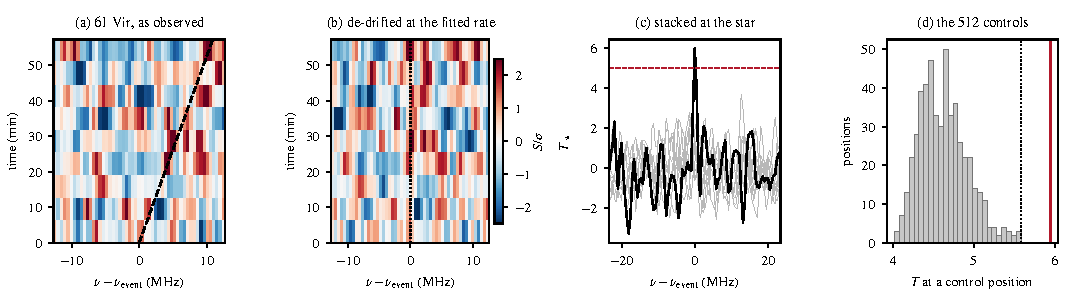
\includegraphics[width=\textwidth]{figures/event_crossings.pdf}
\caption{\textbf{The strongest unattributed crossing of the quality-passing
data, and the control field it leads.} Frequencies are in the star's rest
frame.
\emph{(a)}~The dynamic spectrum at \EvAStar's position around the crossing
at \RqFreqSx\,GHz, observed \EvADate, the fitted drift of
\EvADrift\,Hz\,s$^{-1}$ (observatory frame; \LrFlDriftStar{} in the
star's frame) dashed, \EvANInt{} integrations binned into
\EvANBin{} and plotted in units of each bin's noise.
\emph{(b)}~The same rows shifted by that drift.
\emph{(c)}~The de-drifted stack at the star (black) and at the
\RcNRetCtrl{} control positions with retained dynamic spectra (grey), in
units of its own noise, the trigger dashed. \emph{(d)}~The same statistic at
each of the \NCtrl{} rank-screen control positions: the star (solid) against
the highest control (dotted).}
\label{fig:event}
\end{figure*}

\begin{table}
\centering
\caption{\textbf{Can two crossings be one carrier?} The \TjNPair{} pairs
toward one star with an unattributed member, and each HD~14055 triple
(\S\ref{sec:etacrv}).}
\label{tab:pairs}
\scriptsize
%% GENERATED by pairs_v415.py -- do not hand-edit.
\begin{tabular}{@{}l@{\,}l@{\,}c@{\,}r@{\,}r@{\,}r@{\,}r@{\,}r@{\,}l@{}}
\hline
Star & blocks & new & $\Delta t$ & $\dot\nu_{1\star}$ & $\dot\nu_{2\star}$ & $\Delta\nu$ & miss & one? \\
 & & sess. & (d) & \multicolumn{2}{c}{(Hz\,s$^{-1}$)} & (MHz) & grid & \\
\hline
61~Vir & X822/X82f & yes & 3.00 & $+1092$ & $+3221$ & $+755.4$ & 15 & open \\
J1537$-$3319 & X10359/X398 & yes & 123 & $-2000$ & $+2390$ & $+223.5$ & 3.6 & open \\
CP$-$72~2713 & X4a6d/X502d & no & 0.09 & $-2044$ & $+995$ & $+495.6$ & 1476 & no \\
HD~14055 & X24be0/Xd46 & yes & 1.92 & $+1665$ & $-3823$ & $+512.7$ & 100 & open \\
 & X2b2ee/X3835 & yes & 2.09 & $-2390$ & $+2155$ & $+395.5$ & 55 & open \\
 & X3835/Xd526 & yes & 607 & $+2155$ & $-2563$ & $-640.4$ & -- & open \\
 & X2b2ee/Xd526 & yes & 609 & $-2390$ & $-2563$ & $-244.9$ & -- & open \\
 & X3835/X25c5e & yes & 649 & $+2155$ & $+2611$ & $+338.3$ & -- & open \\
 & X2b2ee/X25c5e & yes & 651 & $-2390$ & $+2611$ & $+733.8$ & -- & open \\
\hline
\end{tabular}

\par\vspace{2pt}
%% GENERATED by triple_r30.py -- do not hand-edit.
\begin{tabular}{@{}l@{~}l@{~}l@{}}
\hline
Triple & constant acceleration & circular orbit \\
\hline
X2b2ee/X3835/Xd526 & misses by 1148 & misses by 133 \\
X2b2ee/X3835/X25c5e & misses by 1139 & misses by 56 \\
\hline
\end{tabular}

\par\vspace{2pt}
{\scriptsize \emph{New sess.}: \emph{yes} where the two blocks belong to
different observing sessions. In the \EvAStar{} pair, block \LrFlBlock{}
holds the field leader of Table~\ref{tab:cand}. Starred rates are in the star's frame, the
observatory's own acceleration removed (observatory frame:
Appendix~\ref{sec:edge}). \emph{Miss}: departure from constant
acceleration, in units of the drift grid's resolution over $\Delta t$; a
dash, a pair that resolution cannot separate. \emph{One?}: whether one
carrier could make both crossings. A pair is \emph{yes} when its miss is
\TjAcceptSig{} or less, which is consistent with one carrier but does not
confirm one, and \emph{open} when it misses by more, or cannot be
separated, but some bounded trajectory inside the drift grid still joins the
two. A pair that no such
trajectory joins is \emph{no}, an \emph{edge} pair has one rate on the
grid's outermost trial, which is then a lower bound, and an \emph{untested}
pair has no block of another session covering the window about it. The
last rows give each triple's miss of its third crossing, predicted from the
first two, in resolutions.\par}
\end{table}

\begin{table}
\centering
\caption{\textbf{The field leader}, the crossing whose stellar statistic
exceeds all \NCtrl{} control positions of its own window
(\S\ref{sec:vistest}).}
\label{tab:cand}
\footnotesize
%% GENERATED by recur_v411.py -- do not hand-edit.
\begin{tabular}{@{}>{\raggedright\arraybackslash}p{0.49\columnwidth}@{~~}r@{}}
\hline
 & 61 Vir \\
\hline
Frequency, stellar frame (GHz) & 346.323236 \\
Drift rate, observatory frame (Hz\,s$^{-1}$) & $+3182$ \\
\quad in the star\textquoteright s frame & $+3221$ \\
$T_\star$ & 5.947 \\
Highest control $T$ & 5.58 \\
Fitted amplitude (mJy) & 118.6 $\pm$ 19.9 \\
Peak-channel EIRP (W) & $5.0 \times 10^{14}$ \\
Repeat epochs measured & 6 \\
Nearest separated epoch, separation (h) & $-24.12$ \\
$T$ expected if it stayed in the cell, $T_{\rm pers}$ & 117.70 \\
$T$ measured, matched drift, $T_{\rm rep}$ & $+2.05$ \\
Amplitude still bounded, $(T_{\rm rep}+5)/T_{\rm pers}$ & 0.06 $S$ \\
Recovery chance $\Phi$ if the amplitude is $5S/T_\star$ ($S$) & 1.00 (1.00) \\
Nearest masked transition & SO($9_{8}$--$8_{7}$) \\
\quad its offset $\Delta v_\star$ (km\,s$^{-1}$) & $-177.6$ \\
Disposition & not confirmed \\
\hline
\end{tabular}

\par\vspace{2pt}
{\scriptsize \emph{Notes.} $S$ is the amplitude of the discovery crossing.
The recovery chance $\Phi$ is given for a carrier of amplitude $\StageNullTrig\,S/T_\star$,
at which the discovery would only just have reached the threshold, and in
parentheses for one at the full discovery amplitude $S$.\par}
\end{table}
